\documentclass[12pt,a4paper]{article}

% ---------- Tiếng Việt, phông ----------
\usepackage[utf8]{inputenc}
\usepackage[T5]{fontenc}
\usepackage[vietnamese]{babel}

% ---------- Trang, khoảng cách ----------
\usepackage[a4paper,left=3cm,right=2cm,top=3.2cm,bottom=2.8cm,headheight=1.4cm,headsep=0.9cm]{geometry}
\usepackage{setspace}
\setstretch{1.3}
\setlength{\parindent}{1.25em}
\setlength{\parskip}{6pt}

% ---------- Hình, bảng, danh sách ----------
\usepackage{graphicx}
\usepackage{float}
\usepackage{subcaption}
\usepackage{caption}
\captionsetup{labelsep=colon,font=normalsize}
\usepackage{enumitem}
\setlist[itemize]{leftmargin=1.5em,itemsep=4pt,topsep=8pt}
\usepackage{xcolor}

% ---------- Tiêu đề mục ----------
\usepackage{titlesec}
\titleformat{\section}{\normalfont\Large\bfseries}{\thesection}{1em}{}
\titleformat{\subsection}{\normalfont\large\bfseries}{\thesubsection}{1em}{}
\titleformat{\subsubsection}{\normalfont\normalsize\bfseries}{\thesubsubsection}{1em}{}
\titlespacing*{\section}{0pt}{6pt}{18pt}
\titlespacing*{\subsection}{0pt}{20pt}{12pt}
\titlespacing*{\subsubsection}{0pt}{16pt}{10pt}

% ---------- Mục lục ----------
\usepackage{tocloft}
\renewcommand{\contentsname}{Mục lục}
\renewcommand{\cfttoctitlefont}{\normalfont\Large\bfseries}
\setlength{\cftbeforetoctitleskip}{0pt}
\setlength{\cftaftertoctitleskip}{24pt}
\renewcommand{\cftsecfont}{\bfseries}
\renewcommand{\cftsecpagefont}{\bfseries}
\setlength{\cftbeforesecskip}{14pt}
\setlength{\cftbeforesubsecskip}{6pt}
\setlength{\cftbeforesubsubsecskip}{6pt}
\setcounter{tocdepth}{3}
\setcounter{secnumdepth}{3}

% ---------- Header, footer ----------
\usepackage{fancyhdr}
\usepackage{lastpage}
\pagestyle{fancy}
\fancyhf{}
\fancyhead[L]{%
  \raisebox{-0.25\height}{
\includegraphics[height=1.0cm]{hinh/logo.png}}\hspace{0.8cm}%
  \begin{tabular}[b]{@{}l@{}}\small\bfseries Trường Đại học Sài Gòn\\ \small\bfseries Khoa Công Nghệ Thông Tin\end{tabular}}
\fancyfoot[L]{\scriptsize BrewLite - Ứng dụng đặt đồ uống \& Thanh toán Online}
\fancyfoot[R]{\scriptsize Trang \thepage/\pageref{LastPage}}
\renewcommand{\headrulewidth}{0.5pt}
\renewcommand{\footrulewidth}{0.5pt}
\fancypagestyle{plain}{}  % trang Mục lục cũng có header/footer như mẫu

% ---------- Khung kết quả chạy lệnh (thay cho ảnh chụp terminal) ----------
\definecolor{nenterm}{RGB}{24,24,24}
\definecolor{chuterm}{RGB}{230,230,230}
\usepackage{fancyvrb}
\usepackage[most]{tcolorbox}
\newtcolorbox{terminal}[1][0.95\textwidth]{colback=nenterm,colframe=nenterm,arc=0pt,boxrule=0pt,
  left=6pt,right=6pt,top=5pt,bottom=5pt,width=#1,before upper=\color{chuterm}}
\fvset{fontsize=\scriptsize}

% ---------- Mẫu một User Story ----------
\newcommand{\userstory}[2]{%
  \noindent\textbf{User Story:}\par
  #1\par
  \hspace*{\parindent}\textbf{Tiêu chí chấp nhận (Acceptance Criteria):}
  \begin{itemize}
    #2
  \end{itemize}}

\usepackage[hidelinks]{hyperref}

% =====================================================================
%  THÔNG TIN BÌA - SỬA Ở ĐÂY
% =====================================================================
\newcommand{\gvhd}{ThS.Từ Lăng Phiêu}
\newcommand{\thanhvien}{%
  Nguyễn Tiến Đạt - 3124410061\\
  Phan Thành Đạt - 3124410065\\
  Trần Anh Trung - 3124410380\\
  Đinh Văn Đạt - 3124410053\\
  Đỗ Chí Thanh - 3124410320\\
  Lê Bảo Trọng Tấn - 3124410316}
\newcommand{\thangnam}{10/2026}

\begin{document}

% =====================================================================
%  BÌA
% =====================================================================
\begin{titlepage}
  \setstretch{1.15}
  \centering
  {\large\bfseries TRƯỜNG ĐẠI HỌC SÀI GÒN\\[2pt] KHOA CÔNG NGHỆ THÔNG TIN\par}
  \vspace{1.2cm}
  
\includegraphics[width=3.2cm]{hinh/logo.png}\par
  \vspace{1.6cm}
  {\Large\bfseries CÔNG NGHỆ PHẦN MỀM\par}
  \vspace{1cm}
  \rule{\textwidth}{0.6pt}\par
  \vspace{0.5cm}
  {\huge\bfseries BrewLite\par}
  \vspace{0.6cm}
  {\LARGE\bfseries Ứng dụng Đặt đồ uống\\[4pt] \& Thanh toán Online\par}
  \vspace{0.5cm}
  \rule{\textwidth}{0.6pt}\par
  \vfill
  \begin{tabular}{@{}r@{\hspace{0.6em}}l@{}}
    \textbf{GVHD:} & \gvhd\\[8pt]
    \textbf{SV:}   & \begin{tabular}[t]{@{}l@{}}\thanhvien\end{tabular}
  \end{tabular}\par
  \vfill
  {\bfseries TP. HỒ CHÍ MINH, THÁNG \thangnam\par}
\end{titlepage}

% =====================================================================
%  MỤC LỤC
% =====================================================================
\setcounter{page}{1}
\tableofcontents
\newpage

% =====================================================================
\section{GIỚI THIỆU}
% =====================================================================
\subsection{Giới thiệu}
Tại các quán cà phê, khách hàng thường phải xếp hàng chờ gọi món và thanh toán vào giờ cao điểm. Việc ghi order và thu tiền thủ công cũng dễ dẫn đến nhầm lẫn đơn hàng và sai sót khi thu ngân.

BrewLite là ứng dụng đặt đồ uống trên nền tảng web theo hướng Mobile-First, phục vụ chi nhánh duy nhất BrewLite An Dương Vương (273 An Dương Vương, Phường 3, Quận 5, TP.HCM). Hệ thống cho phép khách hàng xem thực đơn, tùy chỉnh size, mức đường, mức đá và topping, quản lý giỏ hàng, đặt đơn, thanh toán không tiền mặt qua cổng VNPay (môi trường sandbox) hoặc bằng điểm thưởng, sau đó theo dõi trạng thái đơn và tới quầy đọc mã đơn để nhận món. Mục tiêu là giảm thời gian chờ, hạn chế sai sót và nâng cao hiệu quả phục vụ.

\subsection{Mục tiêu đề tài}
\subsubsection{Mục tiêu tổng quát}
Xây dựng ứng dụng BrewLite hỗ trợ người dùng đặt đồ uống và thanh toán trực tuyến qua cổng VNPay, đồng thời ghi nhận lịch sử đơn hàng, lịch sử giao dịch và điểm thưởng thành viên một cách chính xác, an toàn.

\subsection{Đối tượng sử dụng}
Hệ thống BrewLite hướng đến hai nhóm đối tượng chính:

\subsubsection{Khách hàng}
Khách hàng sử dụng ứng dụng để xem danh sách đồ uống, lựa chọn và tùy chỉnh sản phẩm, đặt hàng, thanh toán qua VNPay hoặc bằng điểm, theo dõi đơn hàng và tích lũy điểm thưởng.

\subsubsection{Nhân viên quầy}
Nhân viên quầy nhận mã đơn khách đọc tại quầy, đối chiếu đơn đã thanh toán và chuyển đơn qua các bước pha chế: đã thanh toán, đang pha chế, sẵn sàng lấy món, hoàn thành. Ở giai đoạn giữa kỳ, thao tác này được mô phỏng bằng nút \textit{Demo (vai trò quầy)} trên trang theo dõi đơn.

\subsection{Phạm vi đề tài}
Đề tài tập trung vào việc xây dựng các chức năng cơ bản của hệ thống đặt đồ uống trực tuyến, bao gồm:
\begin{itemize}
  \item Xem danh sách đồ uống.
  \item Quản lý giỏ hàng.
  \item Đặt hàng trực tuyến.
  \item Thanh toán đơn hàng qua VNPay sandbox hoặc bằng điểm thưởng.
  \item Xem lịch sử đơn hàng và lịch sử giao dịch.
\end{itemize}

\newpage
% =====================================================================
\section{PHÂN TÍCH YÊU CẦU HỆ THỐNG}
% =====================================================================
\subsection{Yêu cầu chức năng (Functional Requirements)}

\subsubsection{Hiển thị danh sách đồ uống (Menu)}
Hệ thống hiển thị danh sách các loại đồ uống hiện có tại cửa hàng BrewLite, bao gồm hình ảnh minh họa, tên sản phẩm, giá bán, số lượt bán và tình trạng còn hàng.

Người dùng có thể lọc theo danh mục, sắp xếp và tìm kiếm món (gõ không dấu hoặc viết tắt, ví dụ \texttt{bx} cho Bạc xỉu) để chọn đồ uống phù hợp với nhu cầu.

\subsubsection{Xem chi tiết và tùy chọn đồ uống}
Người dùng có thể xem thông tin chi tiết của từng sản phẩm, bao gồm tên, hình ảnh, mô tả và giá bán.

Hệ thống cho phép lựa chọn kích thước (S, M, L), mức đường, mức đá, các loại topping và số lượng sản phẩm. Giá tiền được cập nhật ngay theo các tùy chọn mà người dùng đã chọn.

\subsubsection{Quản lý giỏ hàng}
Người dùng có thể thêm đồ uống vào giỏ hàng, thay đổi số lượng, sửa tùy chọn hoặc xóa sản phẩm không còn nhu cầu mua.

Hệ thống tự động cập nhật tổng số lượng và tổng tiền của giỏ hàng. Thông tin giỏ hàng được lưu trên trình duyệt để không mất dữ liệu khi tải lại trang.

\subsubsection{Đăng ký và đăng nhập tài khoản}
Hệ thống cho phép người dùng đăng ký tài khoản bằng họ tên, email và mật khẩu.

Người dùng đăng nhập để sử dụng các chức năng như đặt hàng, thanh toán, theo dõi lịch sử đơn hàng và điểm thưởng.

Hệ thống xác thực người dùng bằng JWT và bảo vệ thông tin tài khoản.

\subsubsection{Đặt hàng trực tuyến}
Sau khi lựa chọn đồ uống, người dùng có thể tiến hành đặt hàng từ giỏ hàng, chọn hình thức nhận món (đến lấy tại quầy hoặc giao tận nơi) và thời gian lấy.

Hệ thống kiểm tra thông tin đơn hàng, số lượng sản phẩm và tình trạng tồn kho trước khi xác nhận.

Khi đặt hàng thành công, hệ thống lưu thông tin đơn hàng ở trạng thái chờ thanh toán (\texttt{PENDING}) cùng các sản phẩm đã đặt.

\subsubsection{Thanh toán trực tuyến}
BrewLite hỗ trợ thanh toán không dùng tiền mặt qua cổng VNPay trong môi trường thử nghiệm (sandbox), hoặc trả bằng điểm thưởng BrewLite.

Sau khi thanh toán thành công, hệ thống kiểm tra chữ ký và số tiền VNPay trả về, cập nhật trạng thái đơn hàng sang \texttt{PAID} và thông báo kết quả cho người dùng.

Trong trường hợp thanh toán thất bại, người dùng được thông báo lý do và có thể thực hiện lại giao dịch.

\subsubsection{Xem lịch sử và chi tiết đơn hàng}
Người dùng có thể xem danh sách các đơn hàng đã thực hiện.

Thông tin hiển thị bao gồm mã đơn hàng, ngày đặt, danh sách đồ uống, tổng số tiền và trạng thái đơn hàng. Người dùng cũng xem được lịch sử giao dịch VNPay (mã giao dịch, ngân hàng, thời gian, mã phản hồi).

Người dùng chỉ có thể xem những đơn hàng thuộc tài khoản của mình.

\subsubsection{Áp dụng mã giảm giá}
Người dùng có thể nhập mã khuyến mãi trong quá trình đặt hàng (ví dụ \texttt{BREW20}, \texttt{VNPAY20}, \texttt{FREESHIP}).

Hệ thống kiểm tra tính hợp lệ, thời hạn sử dụng và điều kiện áp dụng của mã giảm giá (giá trị đơn tối thiểu, phương thức thanh toán, hình thức nhận món).

Nếu mã hợp lệ, số tiền giảm giá được tính vào tổng giá trị đơn hàng.

\subsubsection{Tích lũy điểm thưởng thành viên}
Hệ thống hỗ trợ tích lũy điểm thưởng cho người dùng sau khi hoàn tất thanh toán.

Điểm thưởng được ghi nhận theo quy định của BrewLite: mỗi 1.000đ thanh toán được 1 điểm.

Người dùng có thể theo dõi số điểm, lịch sử điểm và dùng điểm để thanh toán hoặc đổi quà.

\newpage
\subsection{Yêu cầu phi chức năng (Non-functional Requirements)}

\subsubsection{Hiệu năng hệ thống}
Hệ thống BrewLite cần đảm bảo tốc độ phản hồi nhanh và ổn định trong quá trình người dùng thao tác.

Các chức năng như xem danh sách đồ uống, xem chi tiết sản phẩm và quản lý giỏ hàng cần được xử lý nhanh chóng.

API danh sách sản phẩm được đặt mục tiêu phản hồi dưới 1 giây trong môi trường kiểm thử thông thường.

\begin{figure}[H]
\centering
\begin{terminal}[0.85\textwidth]
\begin{Verbatim}
$ for i in 1 2 3 4 5; do curl -s -o /dev/null \
    -w "GET /products lan $i: HTTP %{http_code} - %{time_total}s\n" \
    http://localhost:3001/products; done
GET /products lan 1: HTTP 200 - 0.006290s
GET /products lan 2: HTTP 200 - 0.004042s
GET /products lan 3: HTTP 200 - 0.003544s
GET /products lan 4: HTTP 200 - 0.003554s
GET /products lan 5: HTTP 200 - 0.004111s
\end{Verbatim}
\end{terminal}
\caption{Kết quả kiểm thử hiệu năng hệ thống}
\end{figure}

\subsubsection{Bảo mật hệ thống}
Hệ thống phải đảm bảo an toàn thông tin cá nhân và dữ liệu của người sử dụng.

Mật khẩu được mã hóa một chiều bằng thuật toán băm bcrypt. Các chức năng yêu cầu đăng nhập sử dụng JWT để xác thực.

Hệ thống thực hiện phân quyền, đảm bảo người dùng chỉ có thể truy cập dữ liệu thuộc quyền sở hữu của mình. Kết quả VNPay trả về được kiểm tra chữ ký HMAC-SHA512, nên mọi chỉnh sửa tham số đều bị từ chối.

Dữ liệu đầu vào được kiểm tra để hạn chế các yêu cầu không hợp lệ.

\begin{figure}[H]
\centering
\begin{terminal}[0.95\textwidth]
\begin{Verbatim}
brewlite=# SELECT email, "passwordHash" FROM "User";
      email       |                passwordHash
------------------+---------------------------------------------
 demo@brewlite.vn | $2b$10$xm0wz2g.bJdDH4/p9Dfm3O...

$ curl -X POST http://localhost:3001/auth/register \
    -H "Content-Type: application/json" \
    -d '{"fullName":"A","email":"sai-email","password":"123","confirmPassword":"123"}'
{"message":["Họ tên cần ít nhất 2 ký tự","Email không hợp lệ",
 "Mật khẩu cần có cả chữ và số","Mật khẩu cần ít nhất 8 ký tự"],
 "error":"Bad Request","statusCode":400}

$ curl http://localhost:3001/orders/me        # không gửi JWT
HTTP 401 Unauthorized
\end{Verbatim}
\end{terminal}
\caption{Mật khẩu được băm và dữ liệu đầu vào được kiểm tra}
\end{figure}

\subsubsection{Khả năng sử dụng}
Giao diện BrewLite được thiết kế theo hướng đơn giản, trực quan và dễ sử dụng.

\subsubsection{Tính toàn vẹn dữ liệu}
Hệ thống phải đảm bảo tính chính xác và nhất quán của dữ liệu trong quá trình đặt hàng và thanh toán.

Khi tạo đơn hàng, hệ thống sử dụng transaction và khóa lạc quan (optimistic locking) để việc lưu đơn hàng và trừ tồn kho được thực hiện nhất quán, kể cả khi nhiều khách đặt cùng lúc.

Tổng tiền đơn hàng được tính toán ở phía server nhằm hạn chế việc thay đổi dữ liệu từ phía client.

Quá trình thanh toán sử dụng cơ chế Idempotency (header \texttt{Idempotency-Key}) để tránh xử lý trùng lặp giao dịch.

\begin{figure}[H]
\centering
\begin{terminal}[0.95\textwidth]
\begin{Verbatim}
# Gửi 3 lần POST /payments với cùng Idempotency-Key cho đơn BL677776
{"lan":1,"paymentId":"d3518545-...-8ea13d004c09","status":"PROCESSING"}
{"lan":2,"paymentId":"d3518545-...-8ea13d004c09","status":"PROCESSING"}
{"lan":3,"paymentId":"d3518545-...-8ea13d004c09","status":"PROCESSING"}

brewlite=# SELECT count(*) AS so_giao_dich FROM "Payment"
brewlite-#   WHERE "idempotencyKey" = '338165b5-fb57-4cc3-8b30-ee4e04519fc1';
 so_giao_dich
--------------
            1

$ npm run test:int
PASS test/payments-vnpay.int-spec.ts
PASS test/stock-concurrency.int-spec.ts   # kho 5, 12 khách đặt cùng lúc -> 5 đơn
Tests:       22 passed, 22 total
\end{Verbatim}
\end{terminal}
\caption{Giao dịch sử dụng Transaction, Idempotency}
\end{figure}

\subsection{User Story}
User Story mô tả các nhu cầu và mong muốn của người dùng khi tương tác với hệ thống BrewLite. Mỗi User Story được xây dựng từ góc nhìn của người sử dụng, nhằm xác định chức năng cần phát triển và giá trị mà chức năng đó mang lại.

Bên cạnh đó, mỗi User Story đi kèm với các tiêu chí chấp nhận (Acceptance Criteria), giúp xác định điều kiện để một chức năng được xem là hoàn thành và đáp ứng yêu cầu.

\subsubsection{US-01 - Xem danh mục đồ uống}
\userstory{Là một khách truy cập, tôi muốn xem danh mục đồ uống, để biết các sản phẩm đang được bán tại BrewLite.}{
  \item Khi truy cập trang thực đơn, hệ thống hiển thị danh sách sản phẩm từ API \texttt{GET /products}.
  \item Mỗi sản phẩm hiển thị tên, giá, hình ảnh, số lượt bán và tình trạng tồn kho theo dữ liệu hệ thống.
  \item Khách hàng có thể lọc theo danh mục, sắp xếp và tìm kiếm món.
  \item Trong khi tải dữ liệu, hệ thống hiển thị trạng thái loading.
  \item Nếu không có sản phẩm phù hợp, hệ thống hiển thị thông báo danh mục trống.
  \item Nếu API gặp lỗi, hệ thống hiển thị thông báo lỗi và nút thử lại.
}

\subsubsection{US-02 - Xem chi tiết và tùy chỉnh đồ uống}
\userstory{Là một khách hàng, tôi muốn xem chi tiết và tùy chỉnh đồ uống, để lựa chọn sản phẩm phù hợp với sở thích của mình.}{
  \item Khi chọn một sản phẩm, hệ thống hiển thị thông tin chi tiết, mô tả, size, mức đường, mức đá và topping.
  \item Khách hàng có thể chọn một size cho sản phẩm.
  \item Khách hàng có thể chọn nhiều topping theo quy tắc của sản phẩm.
  \item Khi thay đổi size hoặc topping, hệ thống cập nhật giá tạm tính tương ứng.
  \item Nếu sản phẩm không tồn tại, hệ thống thông báo rằng không tìm thấy sản phẩm.
}

\subsubsection{US-03 - Quản lý giỏ hàng}
\userstory{Là một khách hàng, tôi muốn thêm, cập nhật số lượng và xóa đồ uống trong giỏ hàng, để quản lý những sản phẩm mình muốn đặt.}{
  \item Khi thêm một sản phẩm hợp lệ, sản phẩm được đưa vào giỏ hàng và số trên biểu tượng giỏ hàng tăng lên.
  \item Khách hàng có thể cập nhật số lượng và sửa tùy chọn của sản phẩm trong giỏ hàng.
  \item Khách hàng có thể xóa một sản phẩm khỏi giỏ hàng.
  \item Hệ thống cập nhật tổng số lượng sản phẩm và tổng tiền sau mỗi thay đổi.
  \item Giỏ hàng được lưu trên trình duyệt để duy trì dữ liệu khi tải lại trang.
  \item Khi giỏ hàng trống, hệ thống hiển thị thông báo phù hợp.
}

\subsubsection{US-04 - Đăng ký và đăng nhập tài khoản}
\userstory{Là một khách hàng, tôi muốn đăng ký và đăng nhập tài khoản, để sử dụng các chức năng đặt hàng, thanh toán và quản lý đơn hàng cá nhân.}{
  \item Khách hàng có thể đăng ký bằng họ tên, email và mật khẩu hợp lệ.
  \item Hệ thống từ chối đăng ký nếu email đã được sử dụng.
  \item Mật khẩu phải có ít nhất 8 ký tự, gồm cả chữ và số; mật khẩu xác nhận phải khớp.
  \item Mật khẩu được băm bằng bcrypt trước khi lưu vào cơ sở dữ liệu.
  \item Khi đăng nhập thành công, hệ thống trả về JWT.
  \item Các API yêu cầu xác thực chỉ cho phép truy cập khi người dùng có JWT hợp lệ.
  \item Nếu thông tin đăng nhập không chính xác, hệ thống thông báo lỗi phù hợp.
}

\subsubsection{US-05 - Thanh toán online}
\userstory{Là một khách hàng, tôi muốn thanh toán đơn hàng qua cổng VNPay hoặc bằng điểm thưởng, để hoàn tất việc mua đồ uống mà không cần sử dụng tiền mặt.}{
  \item Khi giỏ hàng có ít nhất một sản phẩm, nút ``Thanh toán ngay'' hiển thị tổng tiền cần thanh toán.
  \item Khách hàng có thể chọn phương thức VNPay (môi trường sandbox) hoặc Điểm BrewLite.
  \item Khi chọn VNPay, hệ thống tạo link thanh toán có chữ ký HMAC-SHA512 và chuyển khách sang cổng VNPay.
  \item Khi VNPay báo thành công, hệ thống kiểm tra chữ ký, số tiền và cập nhật đơn hàng sang trạng thái \texttt{PAID}.
  \item Khi thanh toán thất bại hoặc khách hủy, hệ thống thông báo lý do (mã phản hồi VNPay) và cho phép khách hàng thanh toán lại an toàn.
  \item Nếu thanh toán thất bại, giỏ hàng được giữ nguyên để khách hàng có thể tiếp tục thao tác.
  \item Sau khi thanh toán thành công, hệ thống hiển thị mã đơn hàng, mã giao dịch VNPay, ngân hàng và màn hình xác nhận.
  \item Hệ thống sử dụng \texttt{Idempotency-Key} để tránh xử lý lặp cùng một yêu cầu thanh toán.
  \item Nếu kết quả thanh toán chưa xác định do lỗi kết nối, hệ thống không tự kết luận thành công hay thất bại; khách hàng dùng chức năng ``Kiểm tra lại với VNPay'' để đối soát.
}

\subsubsection{US-06 - Tạo đơn hàng}
\userstory{Là một khách hàng đã đăng nhập, tôi muốn tạo đơn hàng từ giỏ hàng, để đặt mua những đồ uống mình đã lựa chọn.}{
  \item Chỉ người dùng đã đăng nhập mới có thể tạo đơn hàng.
  \item Khách hàng phải có ít nhất một sản phẩm hợp lệ trong giỏ hàng.
  \item Hệ thống kiểm tra thông tin sản phẩm và số lượng tồn kho trước khi tạo đơn.
  \item Nếu sản phẩm không đủ hàng, hệ thống từ chối tạo đơn và thông báo phù hợp.
  \item Backend tự tính tổng tiền dựa trên dữ liệu hợp lệ của sản phẩm và các tùy chọn.
  \item Hệ thống lưu thông tin đơn hàng và chi tiết đơn hàng trong cùng một transaction.
  \item Nếu quá trình tạo đơn thất bại, hệ thống không để lại dữ liệu đơn hàng dở dang.
  \item Sau khi tạo đơn thành công, hệ thống trả về thông tin đơn hàng để khách hàng tiếp tục quy trình thanh toán.
}

\subsubsection{US-07 - Xem lịch sử đơn hàng}
\userstory{Là một khách hàng đã đăng nhập, tôi muốn xem lịch sử đơn hàng của mình, để theo dõi những lần đặt đồ uống trước đây.}{
  \item Khách hàng có thể truy cập danh sách đơn hàng của mình.
  \item Mỗi đơn hàng hiển thị mã đơn, ngày đặt, các món đã đặt, tổng tiền và trạng thái.
  \item Hệ thống chỉ trả về các đơn hàng thuộc về tài khoản đang đăng nhập.
  \item Nếu khách hàng chưa có đơn hàng, hệ thống hiển thị thông báo phù hợp.
  \item Nếu xảy ra lỗi khi tải lịch sử, hệ thống hiển thị thông báo lỗi.
}

\subsubsection{US-08 - Xem chi tiết đơn hàng}
\userstory{Là một khách hàng đã đăng nhập, tôi muốn xem chi tiết đơn hàng, để kiểm tra thông tin đồ uống, số lượng, tổng tiền và trạng thái xử lý.}{
  \item Khách hàng có thể mở chi tiết một đơn hàng thuộc tài khoản của mình.
  \item Hệ thống hiển thị mã đơn hàng, ngày đặt, danh sách sản phẩm, số lượng, giá và tổng tiền.
  \item Hệ thống hiển thị trạng thái hiện tại của đơn hàng và các bước xử lý (đã thanh toán, đang pha chế, sẵn sàng lấy món, hoàn thành).
  \item Nếu đơn hàng không tồn tại hoặc không thuộc quyền sở hữu của khách hàng, hệ thống không tiết lộ thông tin chi tiết của đơn hàng đó.
}

\subsubsection{US-09 - Áp dụng mã giảm giá}
\userstory{Là một khách hàng, tôi muốn áp dụng mã giảm giá cho đơn hàng, để được hưởng ưu đãi khi mua đồ uống.}{
  \item Khách hàng có thể nhập mã giảm giá trong quá trình đặt hàng.
  \item Hệ thống kiểm tra mã giảm giá có tồn tại, còn hiệu lực và đáp ứng điều kiện áp dụng hay không.
  \item Nếu mã hợp lệ, hệ thống tính mức giảm giá theo quy tắc đã cấu hình (phần trăm, mức giảm tối đa, đơn tối thiểu).
  \item Nếu mã không hợp lệ hoặc hết hạn, hệ thống thông báo lý do và không áp dụng ưu đãi.
  \item Backend tự tính lại tổng tiền sau giảm giá.
  \item Tổng tiền đơn hàng không được nhỏ hơn 0.
  \item Số tiền giảm giá không được tùy ý thay đổi bằng dữ liệu do frontend gửi lên.
}

\subsubsection{US-10 - Tích lũy điểm thưởng}
\userstory{Là một khách hàng đã đăng nhập, tôi muốn tích lũy điểm thưởng sau khi thanh toán thành công, để nhận được quyền lợi từ chương trình khách hàng thân thiết.}{
  \item Hệ thống ghi nhận điểm theo quy tắc 1.000đ = 1 điểm.
  \item Chỉ những đơn hàng đã thanh toán thành công (\texttt{PAID}) mới được ghi nhận điểm thưởng.
  \item Mỗi đơn hàng chỉ được cộng điểm một lần.
  \item Nếu hệ thống nhận lại kết quả thanh toán cho cùng một đơn hàng (Return URL và IPN tới cùng lúc), hệ thống không cộng điểm trùng.
  \item Điểm thưởng không được ghi nhận khi thanh toán thất bại.
  \item Nếu không thể ghi nhận điểm, hệ thống xử lý lỗi mà không làm sai lệch số điểm của khách hàng.
}

% =====================================================================
\section{GIAO DIỆN ỨNG DỤNG}
% =====================================================================
\subsection{Tổng quan thiết kế giao diện}
Giao diện BrewLite được định hướng theo phong cách hiện đại, đơn giản và thân thiện với người dùng, sử dụng tông màu nâu cà phê và vàng làm chủ đạo.

Các thành phần giao diện được thiết kế nhằm hỗ trợ khách hàng dễ dàng tìm kiếm đồ uống, thêm sản phẩm vào giỏ hàng và thực hiện thanh toán.

Các màn hình chính của ứng dụng bao gồm:
\begin{itemize}
  \item Màn hình đăng nhập.
  \item Màn hình đăng ký.
  \item Màn hình trang chủ.
  \item Màn hình danh sách sản phẩm.
  \item Màn hình chi tiết sản phẩm.
  \item Màn hình giỏ hàng.
  \item Màn hình thanh toán.
  \item Màn hình cổng thanh toán VNPay (sandbox).
  \item Màn hình thanh toán thành công.
  \item Màn hình lịch sử đơn hàng.
\end{itemize}

\subsection{Giao diện đăng nhập}
Màn hình đăng nhập cho phép người dùng truy cập vào hệ thống thông qua thông tin tài khoản đã đăng ký.

Các thành phần chính:
\begin{itemize}
  \item Ô nhập email đăng nhập.
  \item Ô nhập mật khẩu (có nút hiện/ẩn mật khẩu).
  \item Nút đăng nhập.
  \item Liên kết chuyển sang trang đăng ký.
\end{itemize}

\begin{figure}[H]
\centering
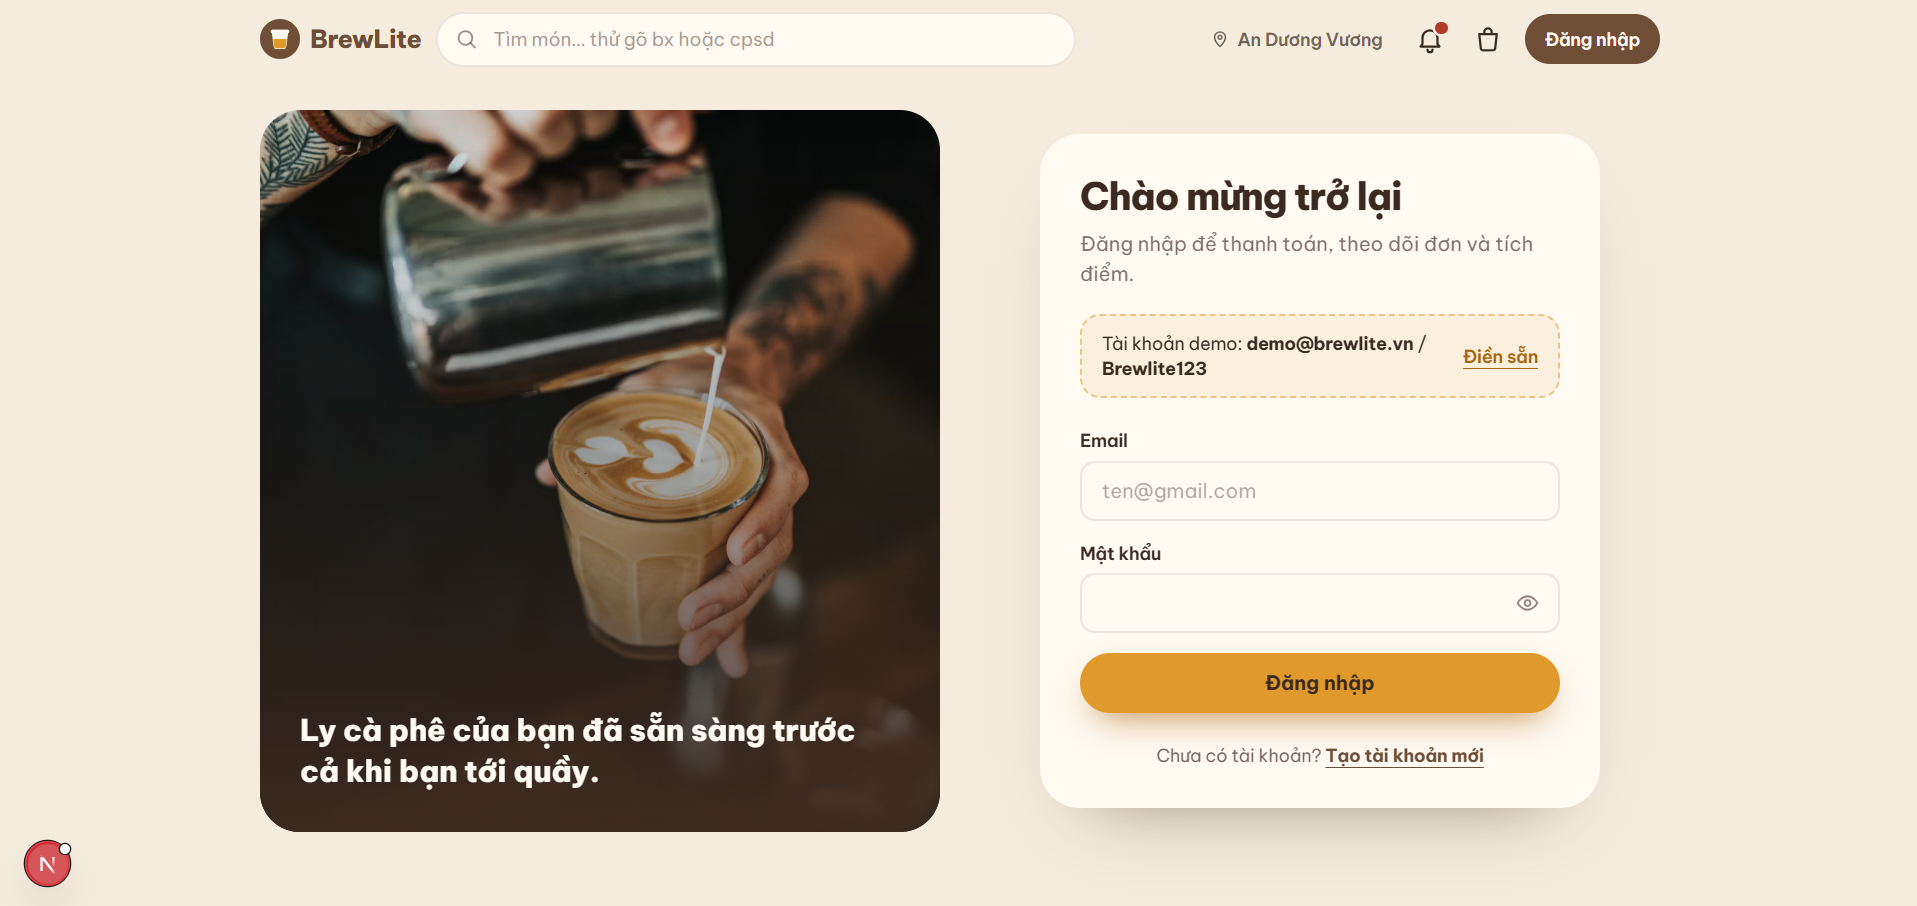
\includegraphics[width=0.75\textwidth]{hinh/02-dang-nhap.png}
\caption{Giao diện đăng nhập BrewLite}
\end{figure}

\subsection{Giao diện đăng ký}
Màn hình đăng ký hỗ trợ người dùng tạo tài khoản mới để sử dụng các chức năng của ứng dụng.

Các thành phần chính:
\begin{itemize}
  \item Nhập họ và tên.
  \item Nhập email tài khoản.
  \item Nhập và xác nhận mật khẩu (có thanh báo độ mạnh mật khẩu).
  \item Nút tạo tài khoản.
\end{itemize}

\begin{figure}[H]
\centering
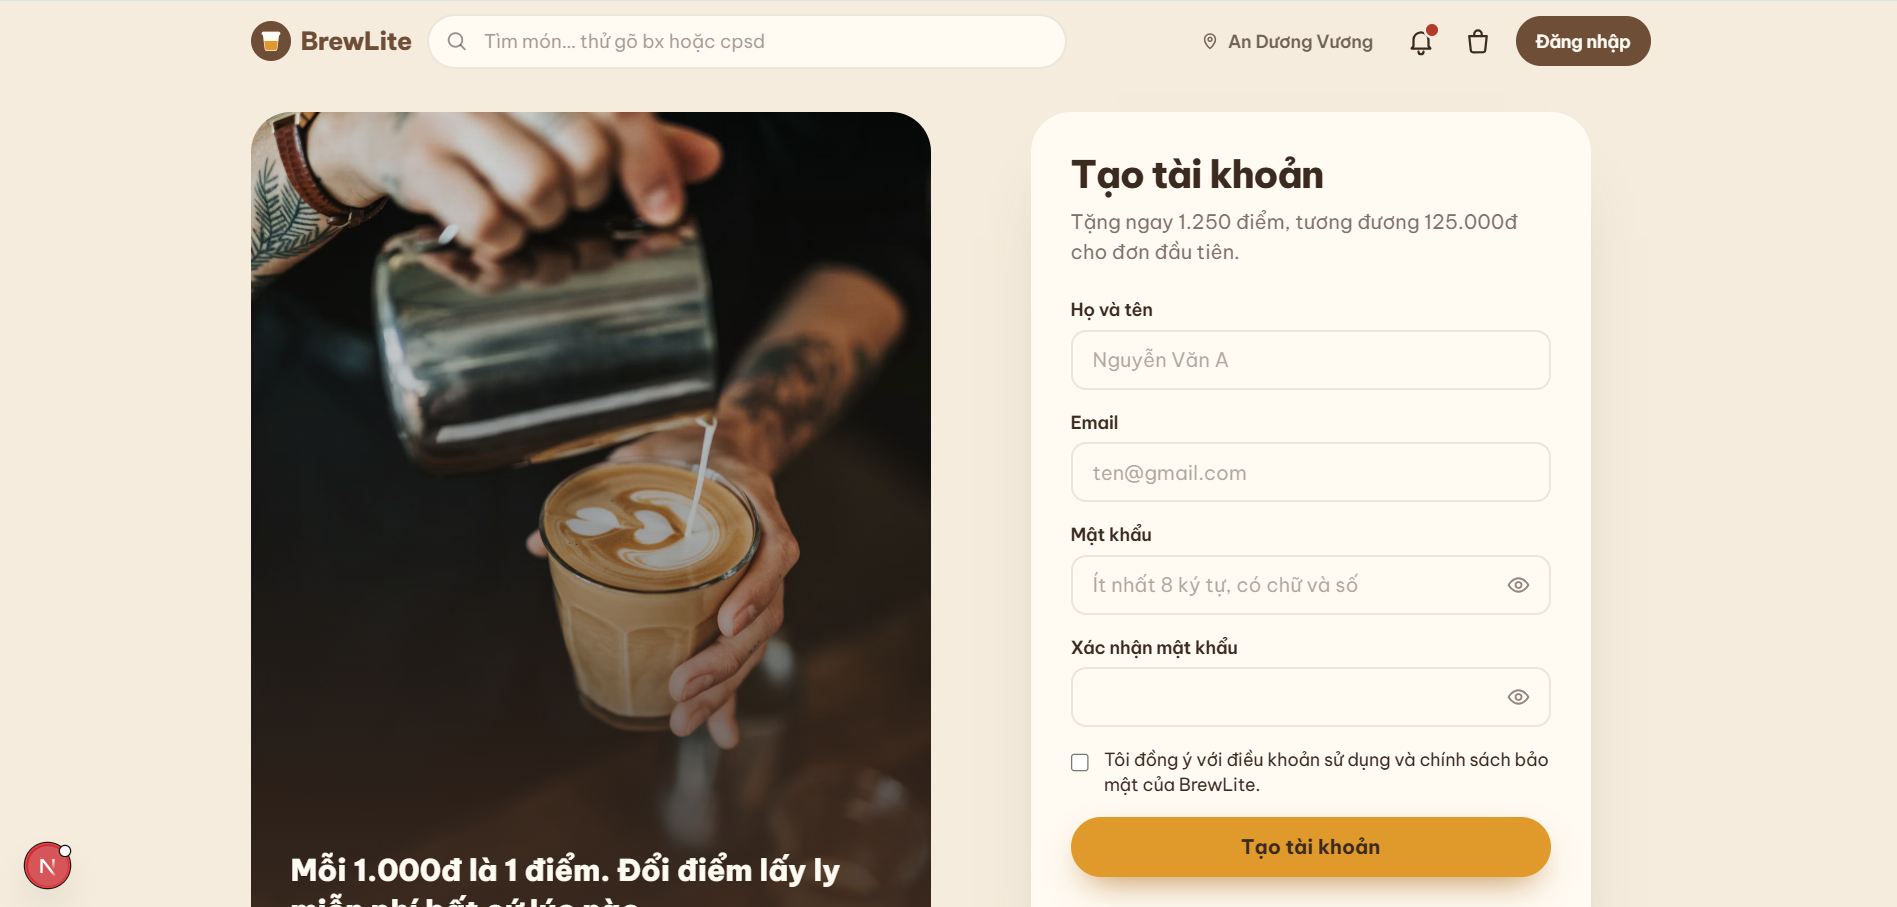
\includegraphics[width=0.75\textwidth]{hinh/03-dang-ky.png}
\caption{Giao diện đăng ký tài khoản}
\end{figure}

\subsection{Giao diện trang chủ}
Trang chủ là màn hình chính sau khi người dùng truy cập ứng dụng.

Màn hình này cung cấp thông tin về các sản phẩm đồ uống, chương trình ưu đãi và các danh mục hiện có.

Các thành phần chính:
\begin{itemize}
  \item Banner ưu đãi đầu trang.
  \item Danh sách sản phẩm theo danh mục.
  \item Thông tin giá, số lượt bán và hình ảnh sản phẩm.
\end{itemize}

\begin{figure}[H]
\centering
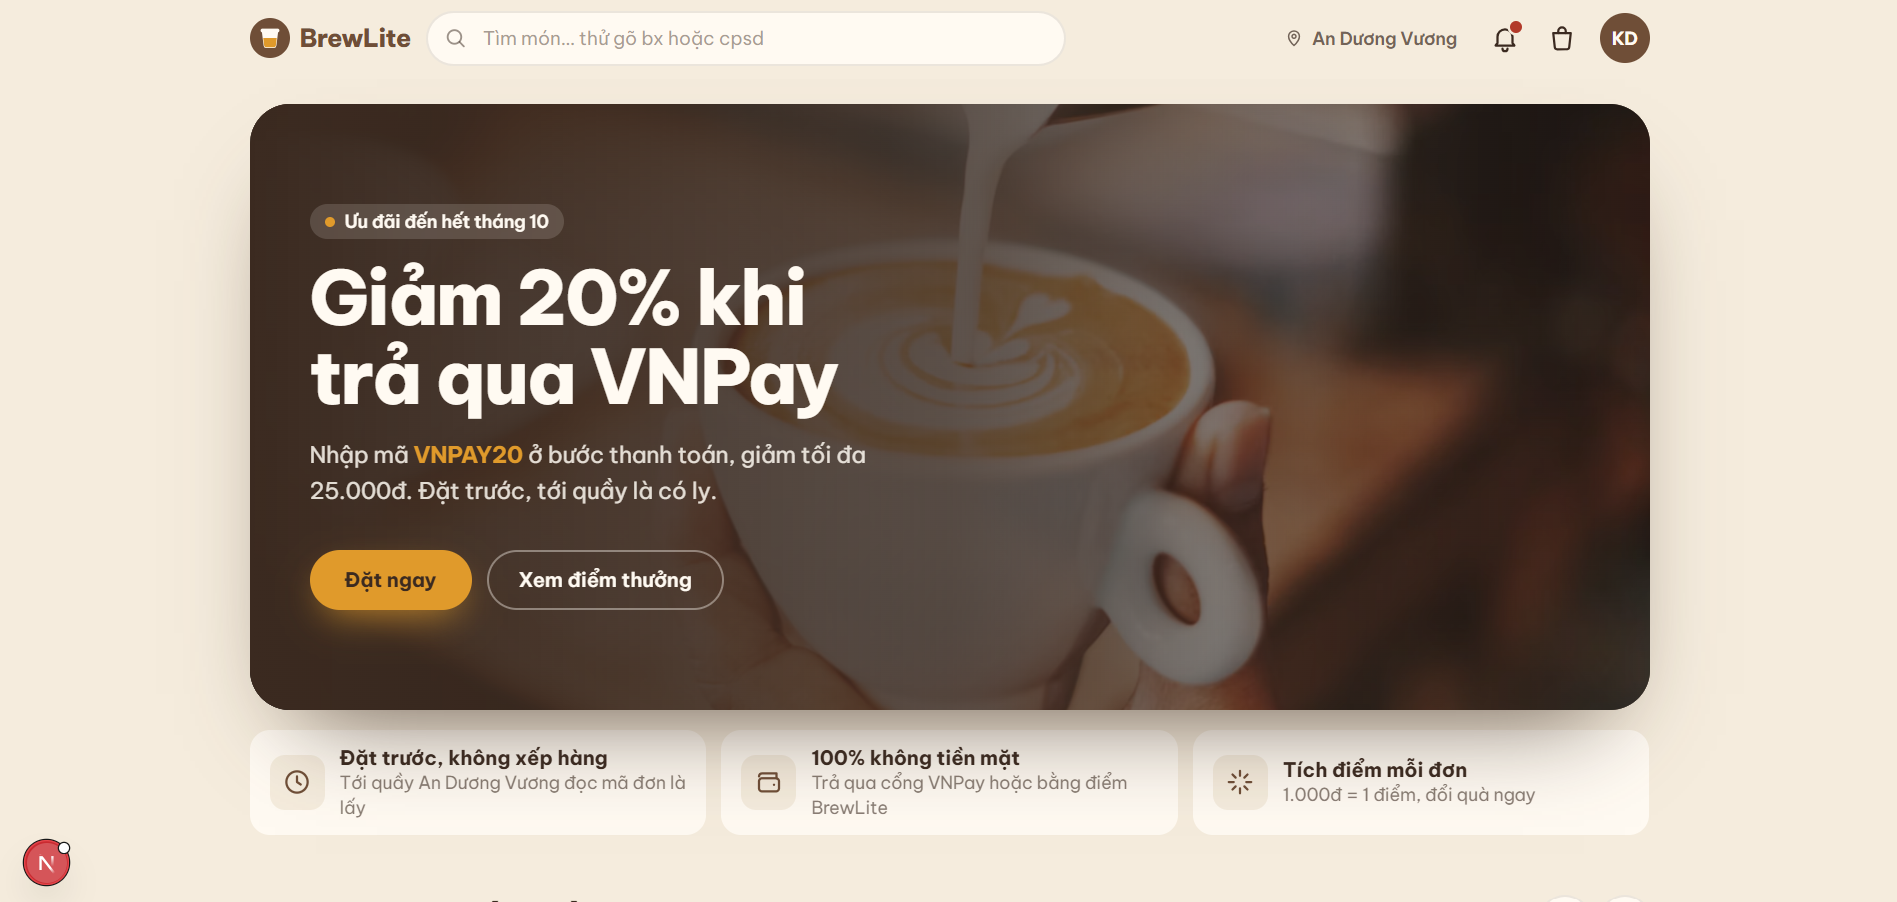
\includegraphics[width=0.49\textwidth]{hinh/04a-trang-chu.png}\hfill
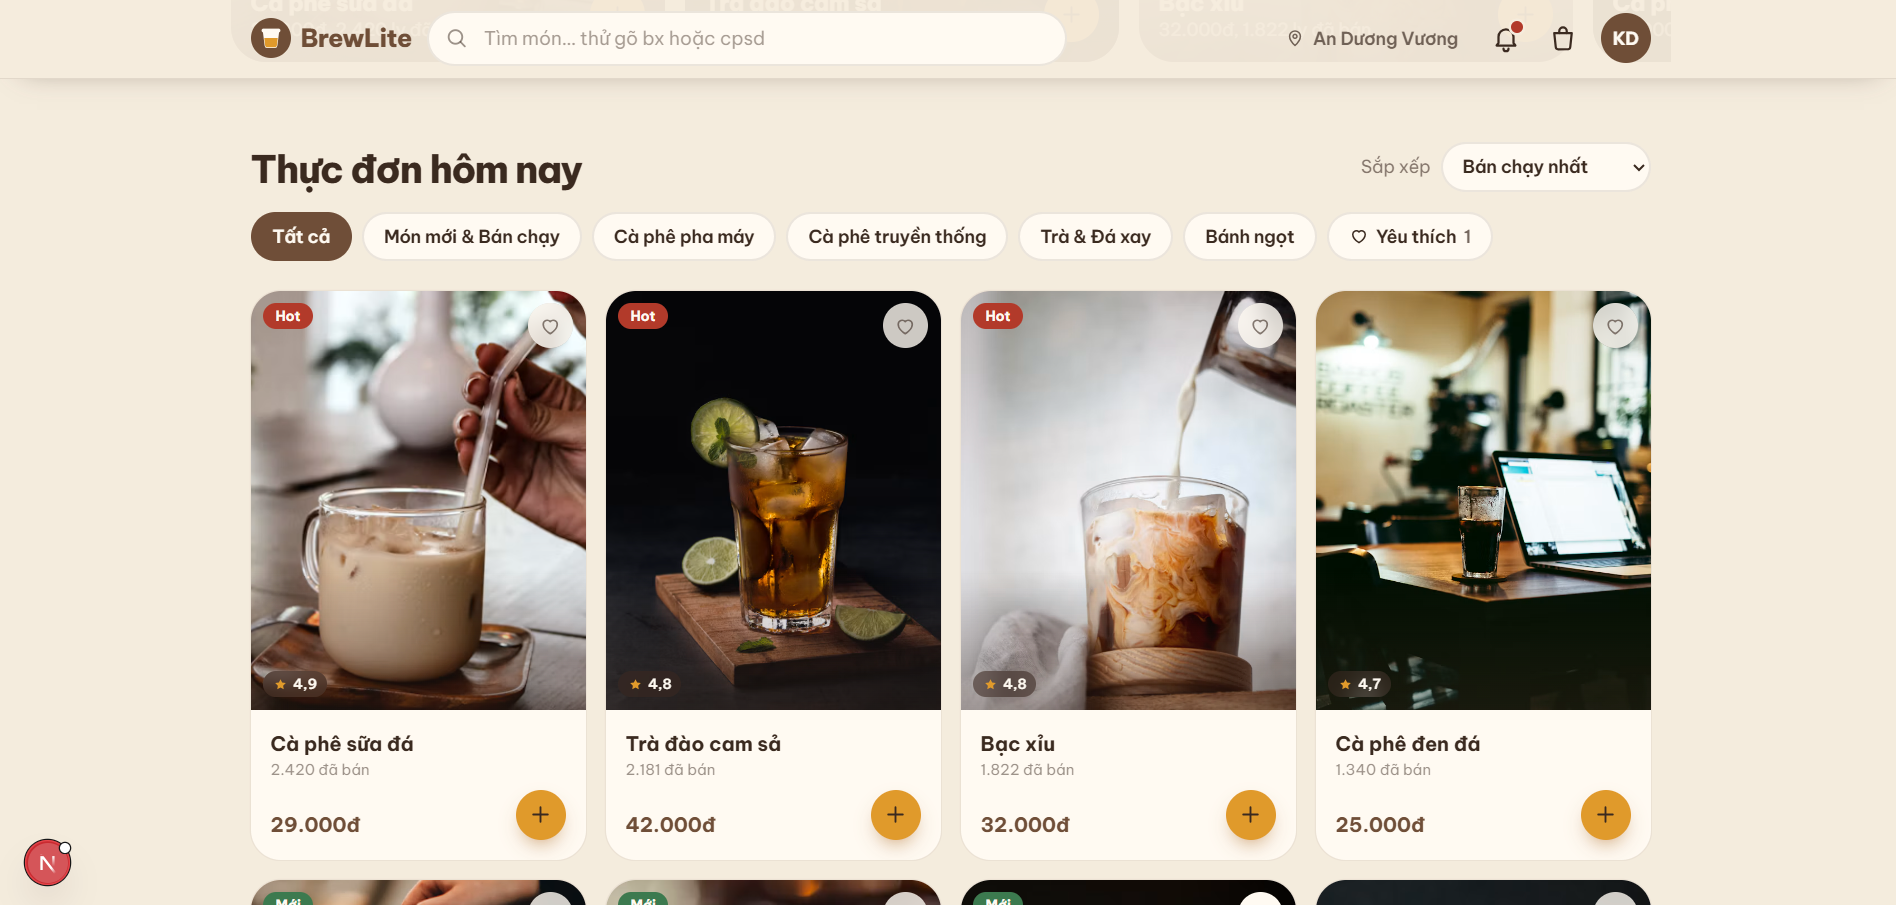
\includegraphics[width=0.49\textwidth]{hinh/04b-thuc-don.png}
\caption{Giao diện trang chủ BrewLite}
\end{figure}

\subsection{Giao diện chi tiết sản phẩm}
Màn hình chi tiết sản phẩm cung cấp thông tin đầy đủ về đồ uống mà khách hàng lựa chọn.

Các thành phần chính:
\begin{itemize}
  \item Hình ảnh đồ uống.
  \item Tên sản phẩm.
  \item Mô tả sản phẩm.
  \item Giá bán.
  \item Lựa chọn size, mức đường, mức đá, topping và số lượng.
  \item Nút thêm vào giỏ hàng.
\end{itemize}

\begin{figure}[H]
\centering
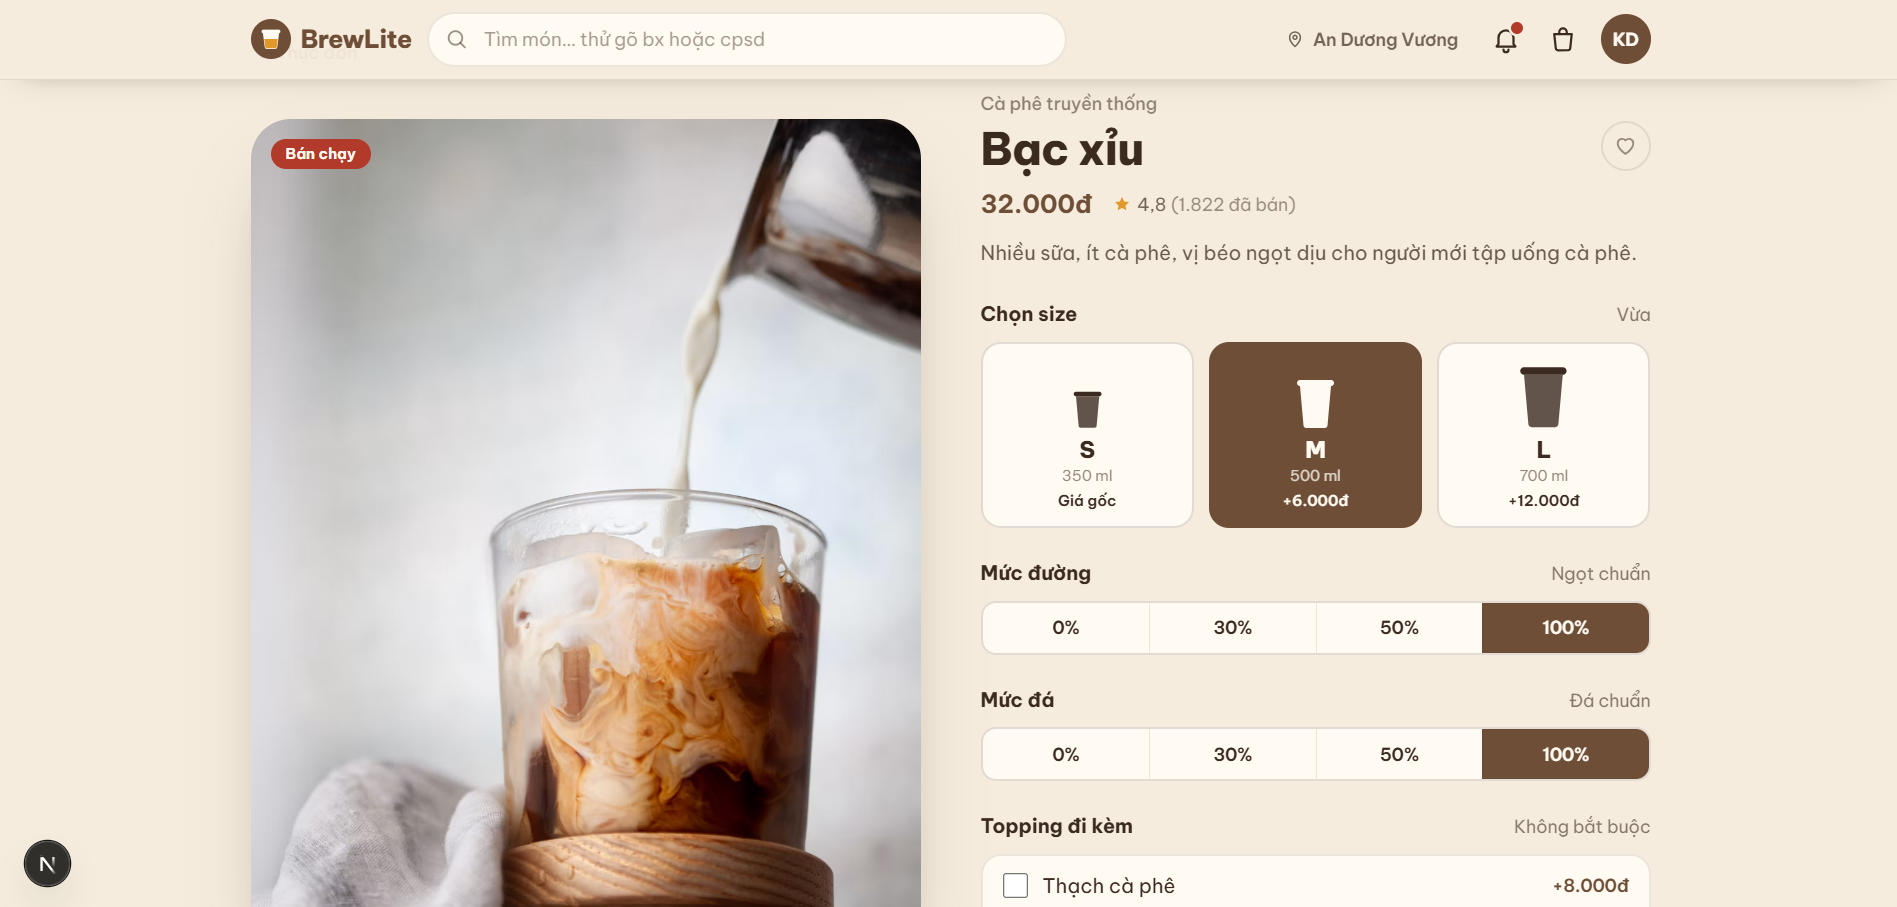
\includegraphics[width=0.75\textwidth]{hinh/05-chi-tiet-mon.png}
\caption{Giao diện chi tiết sản phẩm}
\end{figure}

\subsection{Giao diện giỏ hàng}
Màn hình giỏ hàng cho phép khách hàng kiểm tra và điều chỉnh các sản phẩm trước khi tiến hành đặt hàng.

Các thành phần chính:
\begin{itemize}
  \item Danh sách sản phẩm đã chọn.
  \item Số lượng từng sản phẩm.
  \item Đơn giá và thành tiền.
  \item Chức năng sửa và xóa sản phẩm.
  \item Tổng giá trị đơn hàng.
  \item Nút thanh toán.
\end{itemize}

\begin{figure}[H]
\centering
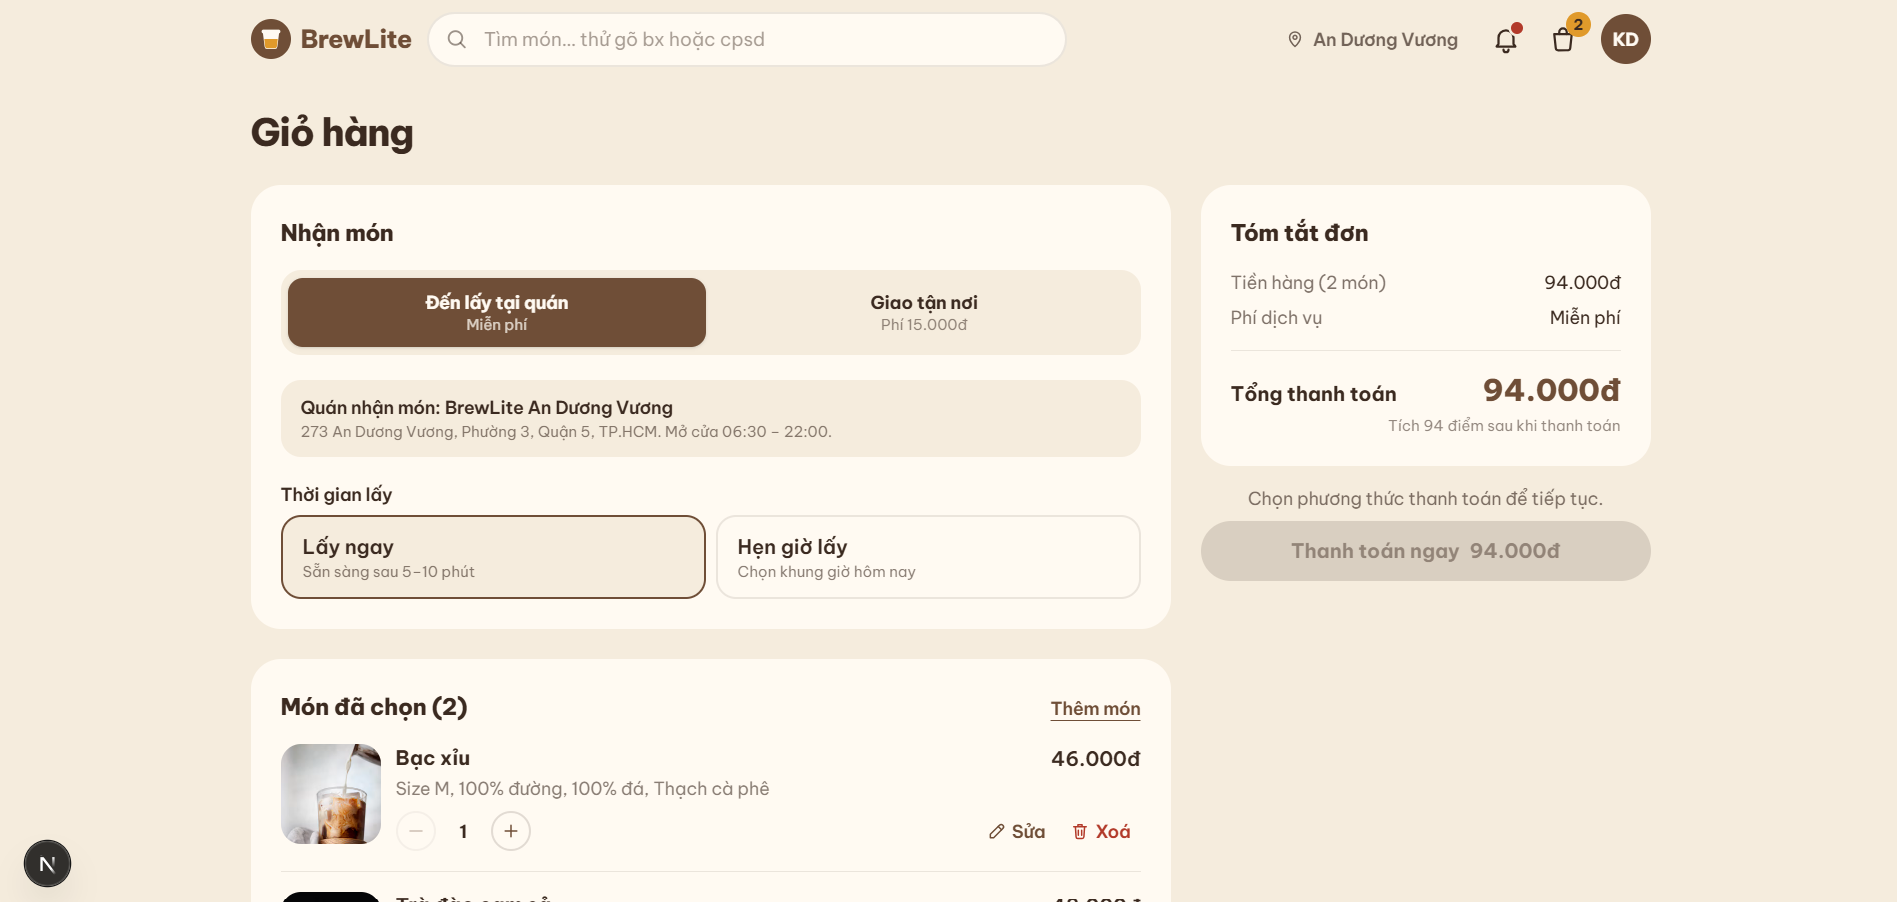
\includegraphics[width=0.75\textwidth]{hinh/06-gio-hang.png}
\caption{Giao diện giỏ hàng}
\end{figure}

\subsection{Giao diện thanh toán}
Màn hình thanh toán cho phép khách hàng kiểm tra thông tin đơn hàng và lựa chọn phương thức thanh toán.

Các thành phần chính:
\begin{itemize}
  \item Thông tin nhận đồ uống (đến lấy tại quầy hoặc giao tận nơi).
  \item Thời gian lấy món.
  \item Tổng số tiền thanh toán.
  \item Phương thức thanh toán: VNPay hoặc Điểm BrewLite.
  \item Ô nhập mã giảm giá.
  \item Nút xác nhận thanh toán.
\end{itemize}

Sau khi giao dịch được xử lý, hệ thống hiển thị thông báo thành công hoặc thất bại tương ứng với kết quả thực tế từ VNPay.

\begin{figure}[H]
\centering
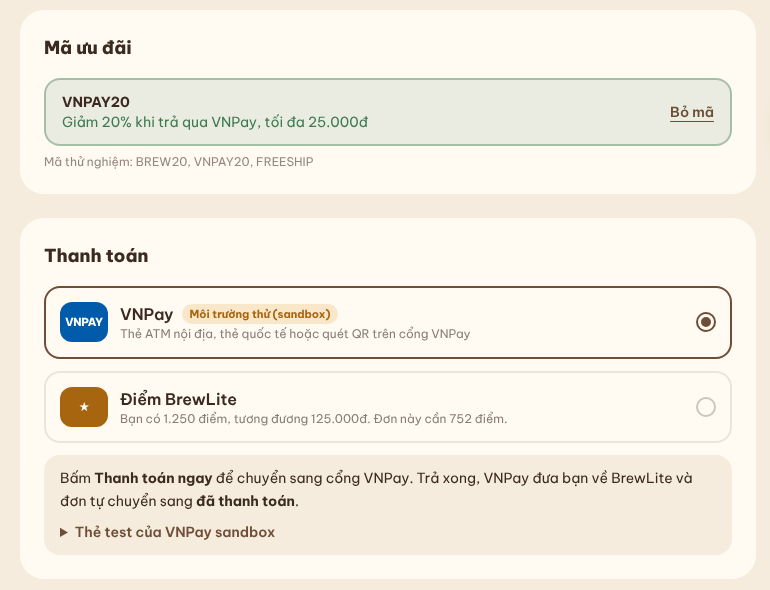
\includegraphics[width=0.49\textwidth]{hinh/07a-thanh-toan.png}\hfill
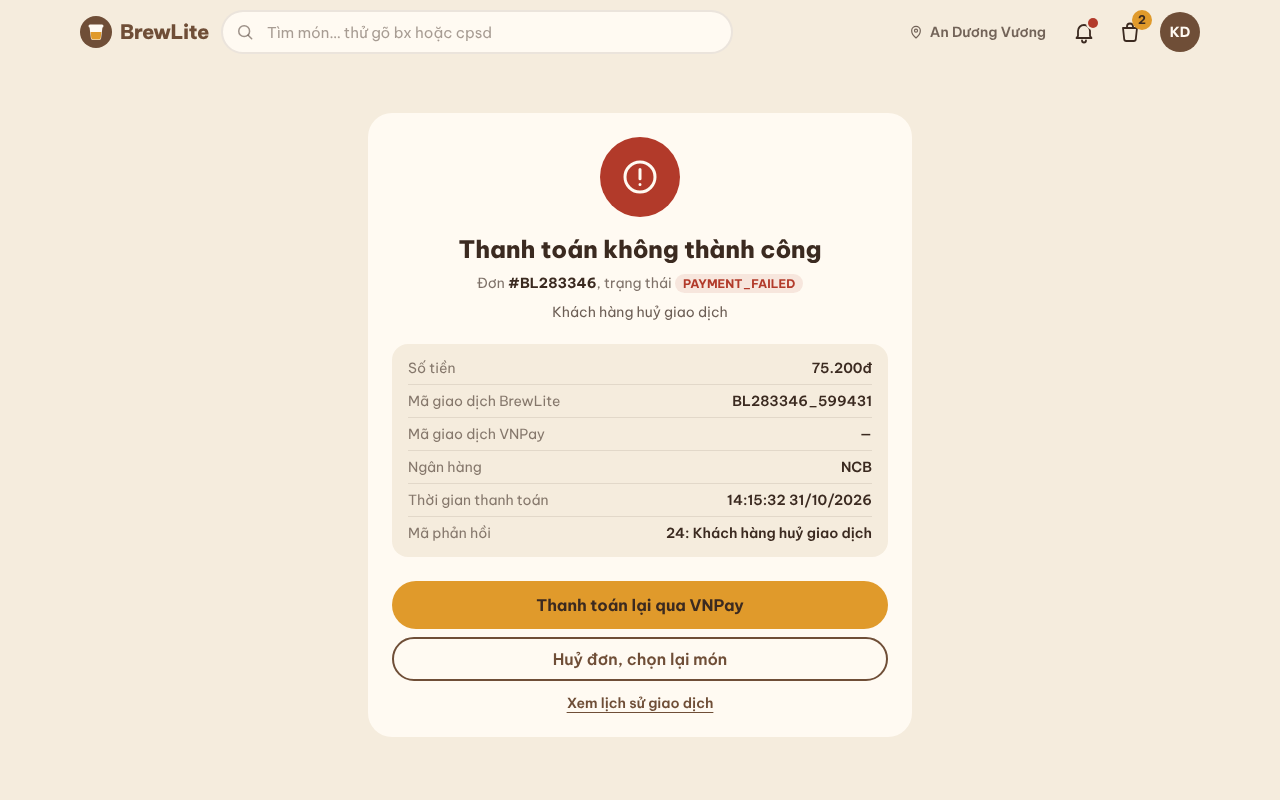
\includegraphics[width=0.49\textwidth]{hinh/07b-thanh-toan-that-bai.png}
\caption{Giao diện thanh toán và thanh toán không thành công}
\end{figure}

\subsection{Giao diện thanh toán qua cổng VNPay (Sandbox)}
Khi khách hàng chọn phương thức VNPay và bấm xác nhận thanh toán, backend BrewLite tạo một đường dẫn thanh toán có chữ ký HMAC-SHA512. Sau đó trình duyệt được chuyển sang cổng thanh toán VNPay. Đề tài dùng môi trường thử nghiệm (sandbox) của VNPay. Môi trường này có giao diện và luồng xử lý giống cổng thật, nhưng chỉ chấp nhận thẻ thử nghiệm và không trừ tiền thật. Vì vậy, các màn hình đều có nhãn \textit{(Test)}.

\subsubsection{Chọn phương thức thanh toán}
Màn hình đầu tiên của cổng VNPay cho khách hàng chọn cách thanh toán.

Các thành phần chính:
\begin{itemize}
  \item Nút \textit{Quay lại} để hủy giao dịch và trở về BrewLite.
  \item App Ngân hàng và Ví điện tử (quét mã VNPAY-QR).
  \item Thẻ nội địa và tài khoản ngân hàng.
  \item Thẻ thanh toán quốc tế.
  \item Ví điện tử VNPAY.
\end{itemize}

Trong quá trình kiểm thử, nhóm dùng lựa chọn \textit{Thẻ nội địa và tài khoản ngân hàng}, sau đó chọn ngân hàng NCB.

\begin{figure}[H]
\centering
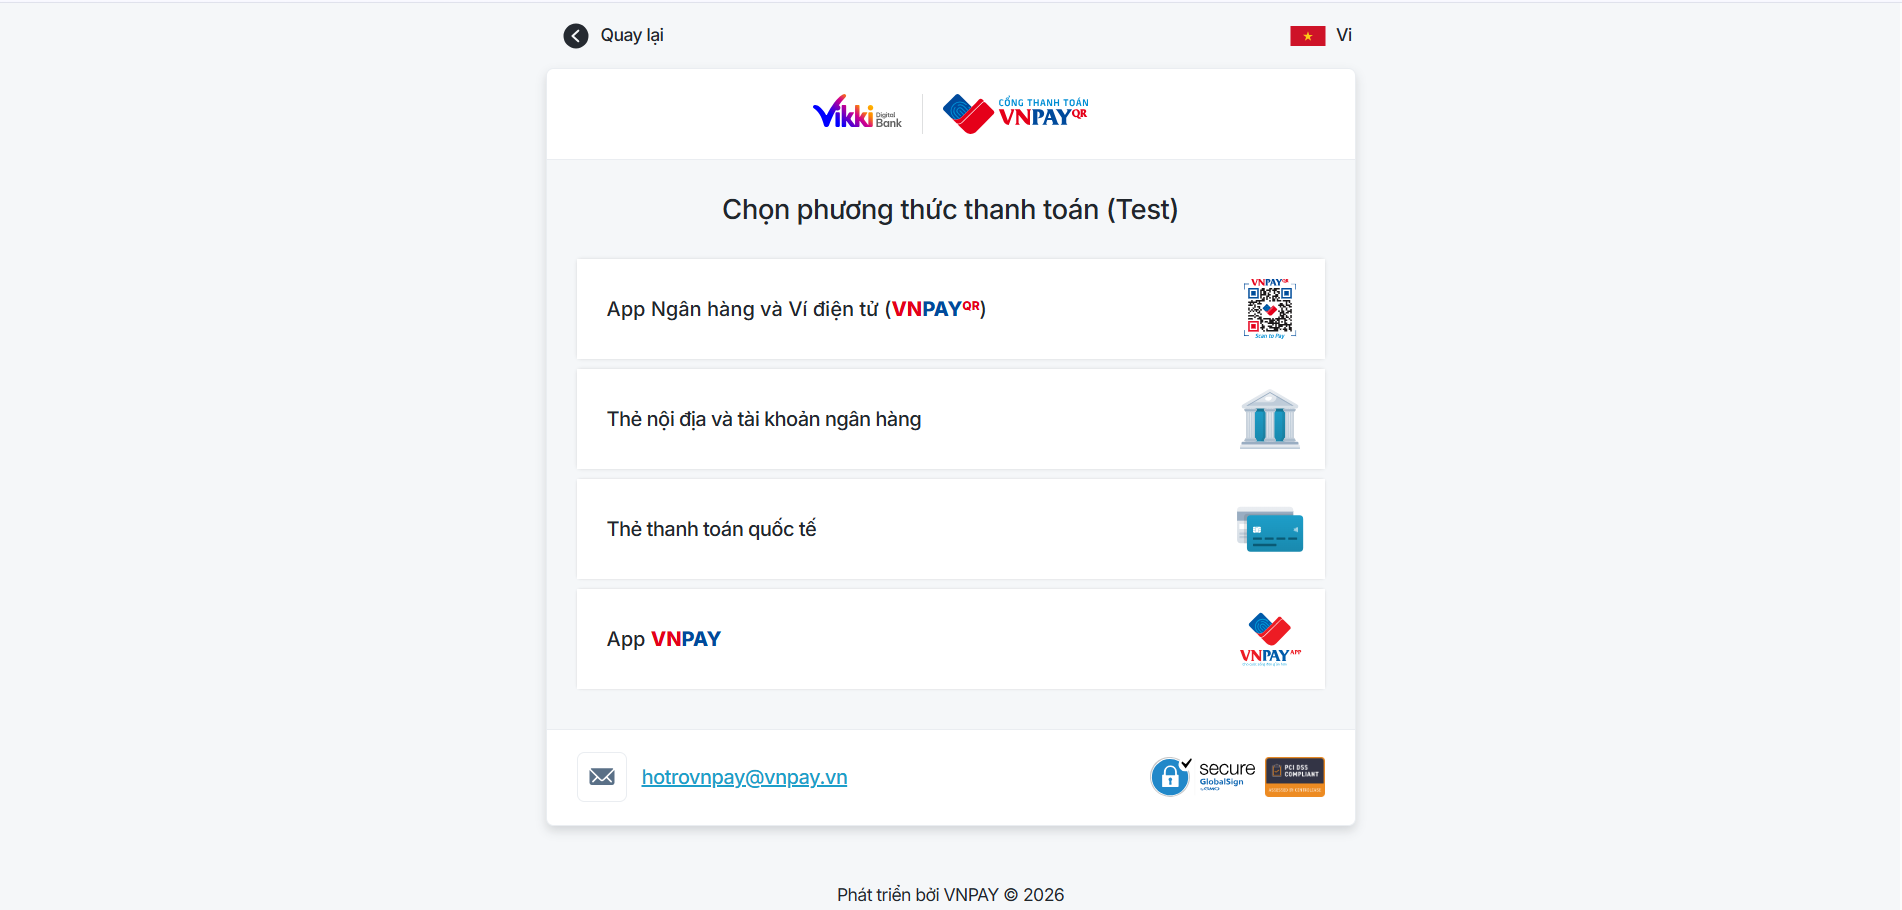
\includegraphics[width=0.85\textwidth]{hinh/07c-trang-thanh-toan-sandbox.png}
\caption{Màn hình chọn phương thức thanh toán trên cổng VNPay sandbox}
\end{figure}

\subsubsection{Thanh toán bằng thẻ nội địa}
Sau khi khách hàng chọn ngân hàng, VNPay hiển thị màn hình nhập thông tin thẻ. Màn hình gồm hai phần.

Thông tin đơn hàng (do BrewLite gửi sang VNPay):
\begin{itemize}
  \item Số tiền thanh toán (ví dụ 94.000đ), đúng bằng tổng tiền do server BrewLite tính.
  \item Giá trị đơn hàng và phí giao dịch.
  \item Mã đơn hàng (mã tham chiếu giao dịch \texttt{vnp\_TxnRef}).
  \item Thời gian còn lại của giao dịch. Khi hết thời gian, giao dịch tự hủy.
\end{itemize}

Thông tin thẻ do khách hàng nhập:
\begin{itemize}
  \item Số thẻ.
  \item Tên chủ thẻ.
  \item Ngày phát hành.
  \item Mã khuyến mại của VNPay (nếu có).
\end{itemize}

Sau khi khách hàng bấm \textit{Tiếp tục}, VNPay yêu cầu nhập mã OTP để xác thực giao dịch.

\begin{figure}[H]
\centering
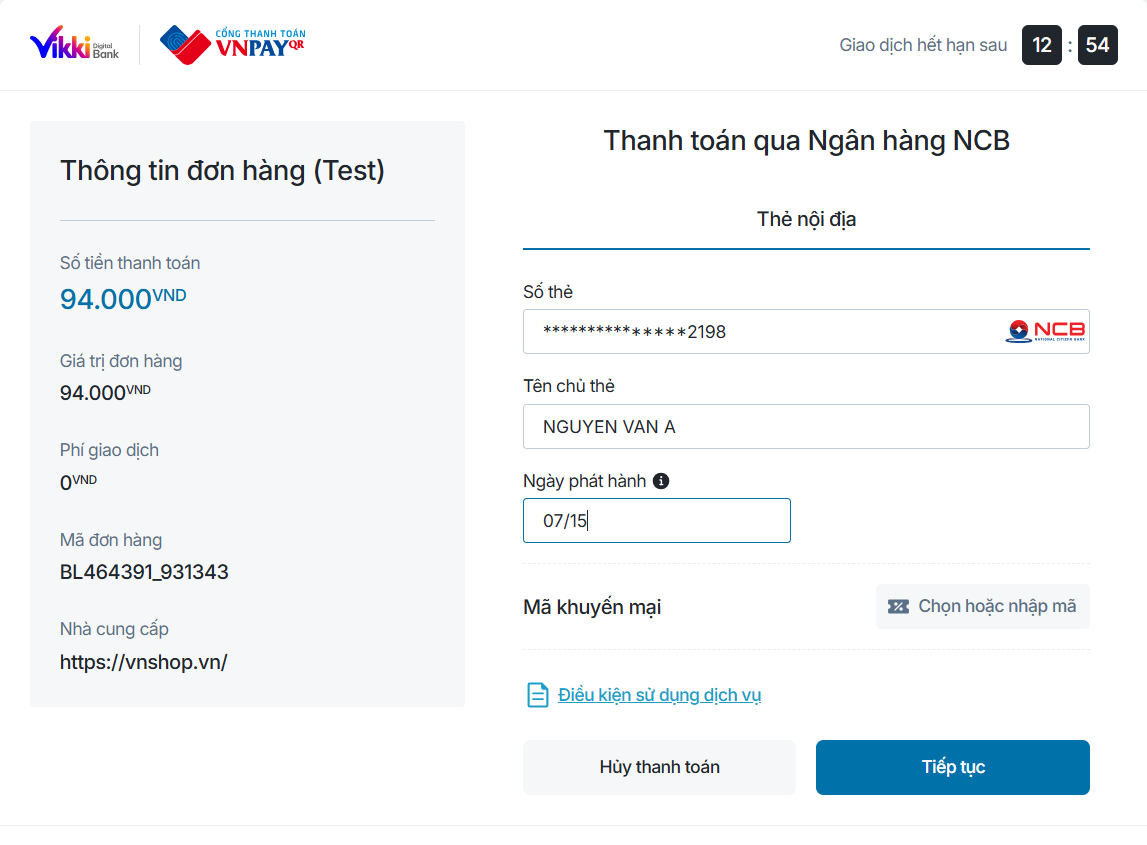
\includegraphics[width=0.85\textwidth]{hinh/07d-thanh-toan-qua-ngan-hang.png}
\caption{Màn hình nhập thông tin thẻ ngân hàng NCB trên VNPay sandbox}
\end{figure}

\subsubsection{Thông tin thẻ thử nghiệm}
Nhóm dùng thẻ thử nghiệm mà VNPay công bố cho môi trường sandbox:

\begin{table}[H]
\centering
\caption{Thẻ thử nghiệm VNPay sandbox}
\begin{tabular}{|l|l|}
\hline
\textbf{Thông tin} & \textbf{Giá trị} \\ \hline
Ngân hàng          & NCB \\ \hline
Số thẻ             & 9704198526191432198 \\ \hline
Tên chủ thẻ        & NGUYEN VAN A \\ \hline
Ngày phát hành     & 07/15 \\ \hline
Mật khẩu OTP       & 123456 \\ \hline
\end{tabular}
\end{table}

\subsubsection{Xử lý kết quả trả về}
Khi giao dịch kết thúc, VNPay gửi kết quả về BrewLite qua hai kênh. Thứ nhất, trình duyệt của khách hàng được chuyển về Return URL. Thứ hai, VNPay gọi IPN trực tiếp từ server của VNPay đến server BrewLite. Khi nhận kết quả, hệ thống:
\begin{enumerate}[leftmargin=1.8em]
  \item Kiểm tra chữ ký \texttt{vnp\_SecureHash}. Nếu sai chữ ký, kết quả bị từ chối.
  \item So sánh số tiền VNPay trả về với tổng tiền của đơn hàng.
  \item Đọc mã phản hồi \texttt{vnp\_ResponseCode}. Mã \texttt{00} nghĩa là thành công, các mã khác là thất bại hoặc khách hàng đã hủy.
  \item Nếu thành công, cập nhật đơn hàng sang \texttt{PAID}, lưu mã giao dịch và ngân hàng, rồi cộng điểm thưởng đúng một lần.
  \item Hiển thị màn hình thanh toán thành công hoặc thất bại tương ứng.
\end{enumerate}

\subsection{Giao diện thanh toán thành công}
Màn hình xác nhận cho khách hàng rằng đơn hàng đã được thanh toán thành công.

Các thành phần chính:
\begin{itemize}
  \item Trạng thái thành công của đơn hàng.
  \item Mã đơn hàng.
  \item Số tiền thanh toán.
  \item Mã giao dịch VNPay, ngân hàng và thời gian thanh toán.
  \item Điểm tích lũy.
  \item Nút theo dõi đơn hàng.
\end{itemize}

\begin{figure}[H]
\centering
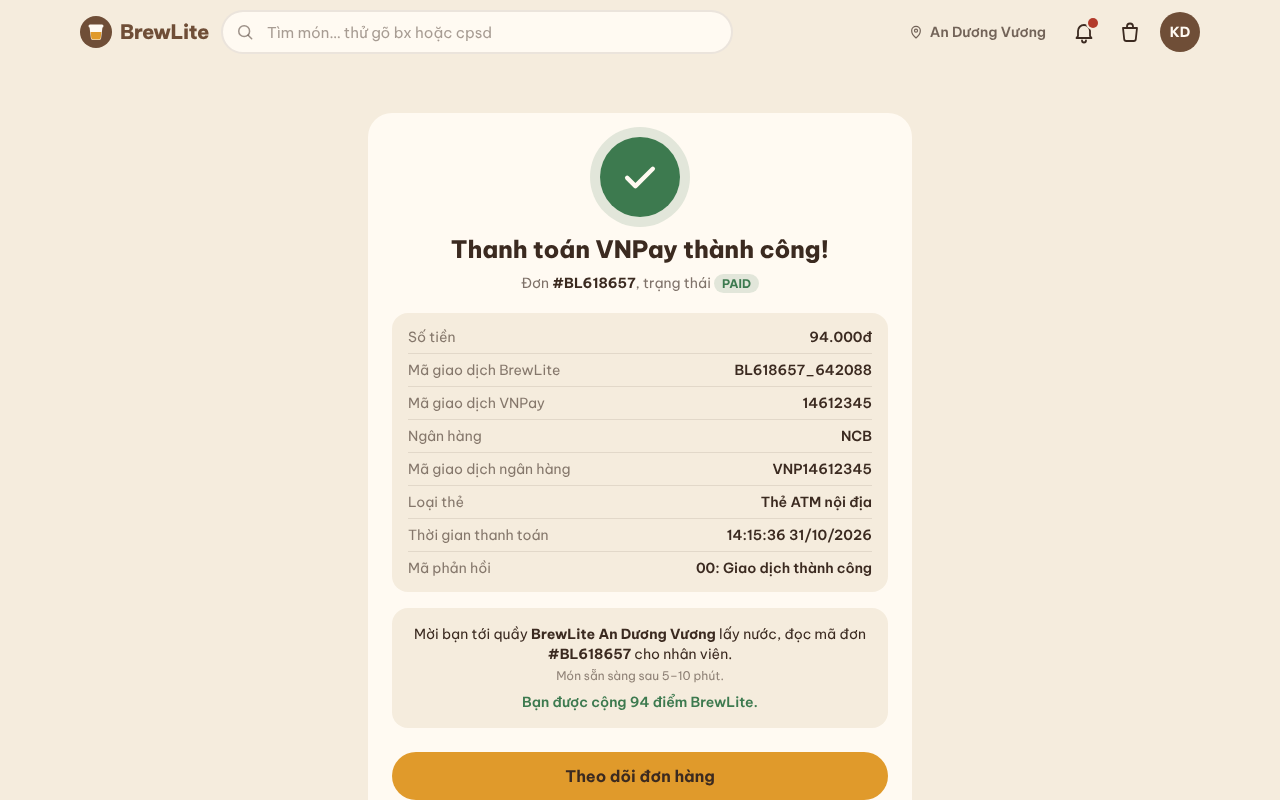
\includegraphics[width=0.75\textwidth]{hinh/09-thanh-toan-thanh-cong.png}
\caption{Giao diện thanh toán thành công}
\end{figure}

\subsection{Giao diện lịch sử đơn hàng}
Màn hình lịch sử đơn hàng giúp người dùng theo dõi các đơn hàng đã thực hiện.

Các thành phần chính:
\begin{itemize}
  \item Danh sách đơn hàng.
  \item Mã đơn hàng.
  \item Ngày đặt hàng.
  \item Tổng giá trị đơn hàng.
  \item Trạng thái đơn hàng.
\end{itemize}

\begin{figure}[H]
\centering
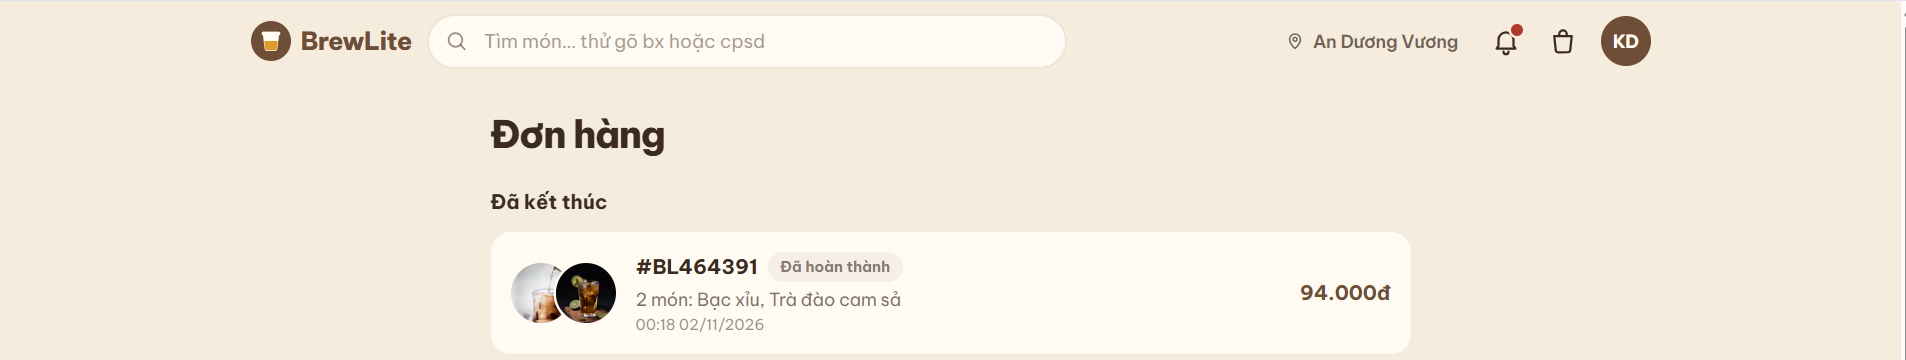
\includegraphics[width=0.75\textwidth]{hinh/08-lich-su-don.png}
\caption{Giao diện lịch sử đơn hàng}
\end{figure}

\end{document}